\section{State of the art}

% Reading list:
% 	- Pitfalls
% 	- Wu
% 	- Powerful
% 	- Hamilton repr learn
% 	- Hamilton graphSage
% 	- GGNN

% ML in graphs intro 

Many data can be represented as a graph, a data structure employed often in computer science and related fields, in fields like biochemistry, social networks, recommender systems and even computer program analysis. Many machine learning applications are created to make predictions using graph-structured data. The way to incorporate the information from graph-structured data as an input to a machine learning model is not straightforward. The fact that graph-structure data is high-dimensional and non-Euclidean are the main barriers for creating a unified and general way to use it as an input to a model. Graph data is irregular, with variable size and variable number of neighbors. Many approaches to transform graph data into usable features for machine learning models exist by using summary graph statistics, kernel functions, or hand-engineered features. Those approaches lack the flexibility to adapt during the learning process.


% Graph Neural Network quick definition (Hamilton, Wu, GGNN, Hamilton, Powerful, PItfalls)
% 	Graph/Subgraph/Node representation idea -> low dimensional embedding (Hamilton)

The idea behind graph neural networks is to learn a mapping that embeds nodes, or entire subgraphs, as points in a low-dimensional vector space $R^d$. The goal is to optimize this mapping so that geometric relationships in the embedding space reflect the structure of the original graph. Previous approaches to learn on graphs used this approach as a preprocessing step, with fixed and/or hand engineered parameters. The graph neural networks treat this representation learning task as a machine learning task itself, using a data-driven approach to learn the embeddings that encode the desired graph structure.

This section will present the main advances in graph neural networks, showing the techniques for representing nodes and entire subgraphs.

\subsection{Notation}

% 	Graph definition (Wu)
\textbf{Definition of a Graph:} A graph is defined as $G = (V,E,A)$ where $V$ is the set of nodes, $E$ is the set of edges and $A$ is the adjacency matrix. In a graph, let $ v_{i} \in V $ denote a node and $ e_{i,j} = (vi, vj) \in E $ denote an edge. The adjacency matrix A is a N x N matrix with $A_{i,j} = w_{i,j} > 0$ if $e_{i,j} \in E$ and $A_{i,j}=0$ if $e_{i,j} \notin E$. The degree of a node is the number of edges connected to it, formally defined as $ degree(v_i) = \sum A_{i,:}$

A graph can be associated with node attributes X, where $X \in R^{N \times D}$ is a feature matrix with $X_i \in R^{D}$ representing the feature vector of node $v_i$. %In the case of $D = 1$, we replace $x \in R^N$ with X to denote the feature vector of the graph.

\textbf{Definition of a directed graph:} A directed graph is a graph with all edges pointing from one node to another. For a directed graph, $A_{i,j} \notequal A_{j,i}$. An undirected graph is a graph with all edges undirectional. For an undirected graph, $A_{i,j} = A_{j,i}$.


% 	Euclidean space definition (Wu, Powerful,pitfalls)
\textbf{Euclidean space:}  a space in any finite number of dimensions, in which points are designated by coordinates (one for each dimension) and the distance between two points is given by a distance formula.  A distance $d$ is defined as a function, let $x,y \in \mathbb{R}^p$:
$$d:\mathbb{R}^{2p} \to \mathbb{R}_{+} \begin{cases}

d(x,y)>0 & \forall x \neq y \\
d(x,y)=0 & iff \quad x=y \\
d(x,y) \leq d(x,z)+d(z,y) & \forall x,y,z

\end{cases}$$

An Euclidean distance $d$ between two points x and y is defined as $d^2(x,y)=(x-y)^T\matchcal{A}(x -y)$ where $\mathcal{A}$ is a positive definite matrix, called a metric.

% 	Non-Euclidean space definition (powerful, pitfalls)
Graph-structured data is considered to be non Euclidean for many reasons. First, there's not a clear definition of the norm of a vector, and so the distance between two nodes has to be defined on some other criteria. Usually the distance between two nodes is computed as the number of nodes that exist in the shorted path following edges between the node at the origin and the node at the destination. 
Second, the distance between nodes, when computed that way, does not fulfill the triangle inequality (3rd condition in the previous definition). Finally, the similarity between nodes, as computed based on the node's attributes, does not need to comply with node distances (as defined by previous sentence ).


\subsection{Early model}

%First Papers, 2005 and 2009, small summary (Wu, Pitfalls)
%	convergence methods
%		- propagation of neighbor information

The idea of a graph neural network was first developed by Gori et al.(2005) \cite{gori} and then by Scarselli et al. (2009) \cite{scarcelli}. Good and generic definitions of the process of training a Graph Neural Network are explained at \cite{hamilton} and \cite{powerful}. They are summarized in the following paragraphs. 

% generalised definition (Powerful)
\textbf{Graph Neural Networks:} GNNs use the graph structure and node features $X_v$ for $v \in V$ to learn a representation vector of a node, $h_v$, or the entire graph $h_{G}$. Modern GNNs follow a neighborhood aggregation strategy, where they iteratively update the representation of a node by aggregating representations of its neighbors. After $k$ iterations of aggregation, a node's representation captures the structural information within it's $k$-hop network neighborhood. Formally, the $k$-th layer of a GNN is:
$$ a_v^{(k)} = AGGREGATE^{(k)}(\{ h_u^{(k-1)} : u \in N(u) \}) , h_v^{(k)} = COMBINE^{(k)}(h_v^{(k-1)}, a_v^{(k)}),$$

where $h_v(k)$ is the feature vector of node $v$ at the $k$-th iteration/layer. The initialization consists in $h_v^{(0)} = X_v$, and $N(v)$ is a set of nodes adjacent to $v$. 
The iterative aggregation process is computationally intensive. modern implementations try to speed up this convergence process, for example by limiting the number of iterations or by using random walks for processing the neighborhood.

% 2 tasks
There are two types of tasks, where GNNs are used: node classification/regression and graph classification/regression.  Node classification or regression is when each node $v \in V$ has an associated label or target value $y_v$ and the goal is to learn a representation vector $h_v$ of $v$ such that $v$'s label or target values can be predicted as $y_v=f(h_v)$. Graph classification or regression is when given a set of graphs $\{ G1, ..., G_N\}$ and their labels or target values $\{y_1,...,y_N\}$ the goal is to learn a representation vector $h_G$ that helps to predict the label or target value of the entire graph $y_G=g(h_G)$.

For node classification/regression, the node representation $h_v^{(K)}$ of the final iteration is used for prediction. For graph classification/regression, the READOUT function aggregates node features from the final iteration to obtain the entire graph's representation $h_G$:
$$h_G = READOUT(\{h_v^{(K)} | v \in G\})$$
The READOUT function can be a simple permutation invariant function such as a summation or a more sophisticated graph-level pooling function.

The choice of $AGGREGATE^{(k)}(\dot)$ and $COMBINE^{(k)}(\dot)$ is crucial. In the next subsection the main evolutions of this model is explained. The main idea is what choices of $AGGREGATE^{(k)}(\dot)$ and $COMBINE^{(k)}(\dot)$  have been used for those state-of-the-art models. 


% slidesCambdribe kipf visual plot of the GNN
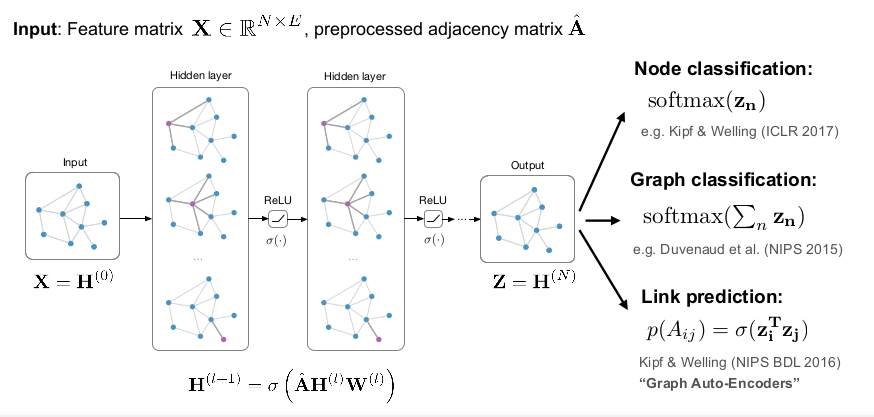
\includegraphics[scale=0.5]{./img/GNN-schema.png}\\[2cm] 


% comment (review and remove redundancy) FOR INTRO

% It follows a recursive neighborhood aggregation framework (also called message passing), where the representation vector of a node is computed by recursively aggregating and transforming feature vectors of its neighboring nodes. After k iterations, a node is represented by its transformed feature vector, which captures the structural information within the node's k-hop network neighborhood. This approach works when the learning task requires to represent each node of the graph, for example for node attribute regression or node classification. When the learning task requires to compute representations at the graph or subgraph level, pooling mechanisms like addition or other aggregations of all the nodes of the (sub)graph are used. 


% In these publications about graph neural networks, they implement models for learning a node's representation by propagating neighbor information in an iterative manner until convergence in all nodes is reached. This process is computationally intensive, modern implementations try to speed up this convergence process, for example by limiting the number of iterations or by using random walks for processing the neighborhood.




\subsection{Advanced models} 





% spatial versus spectral methods----------------(Wu)
Early models try to learn a node's representation by propagating neighbor information in an iterative manner until convergence in all nodes is reached. This process is computationally intensive and so recently there has been several publications that try to make this process less costly. A large number of methods apply the characteristics of convolutional networks in the computer vision domain to graph data. They are called Graph Convolutional Networks (GCN).

\textbf{Graph Convolutional network:}


% Spectral graph theory approaches (Wu)%(Tkipf)
% Spatial based methods (Wu)

The first GCN model is presented in Bruna et al.(2013) \cite{bruna} which develops a variant of graph convolution based on spectral graph theory. There have been several other publications on spectral-based graph convolutional networks \cite{deferrard}. Spectral methods usually handle the whole graph simultaneously and are difficult to parallelize or scale to large graphs. 

There is another kind of convolutional approach for graphs, called spatial-based graph convolutional networks, see \cite{graphsage} and \cite{geometricdl}. These methods directly perform the convolution in the graph domain by aggregating the neighbor nodes' information. Together with sampling strategies, the computation can be performed in a batch of nodes instead of the whole graph, which improves efficiency.

% GNN definitoni form kipf web -----------------------
% Kipf web page: Weisfeiler Lehman  and GCN comparison


The previous subsection showed that the updating of a node state, that is the current value of its attributes, can be formalized as a function of the node states and the aggregation of the neighbor nodes states:

 $$ h_v^{(k)} = COMBINE^{(k)}(h_v^{(k-1)}, a_v^{(k)})$$,

where $a_v^{(k)}$ is the aggregation of the neighborhood. This same concept can be expressed in matrix notation with the adjacency matrix and matrix of weights in the following equation:


$$H^{(k)} = f(H^{(k-1)},A) =  \sigma(AH^{(k-1)}W^{(k-1)}),$$

where $W^{(k)}$ is a weight matrix for the l-th neural network layer and $\sigma(·)$ is a non-linear activation function like ReLU. Some additional constraints must be imposed on the adjacency matrix A. First, it must be added to the identity I, in order to create self-loops and allow the node attributes to be counted in the updating. Second, A must be normalized.

This can then follow the Weisfeiler-Lehman algorithm on graphs, which is used to detect isomorphisms. It assigns a unique set of features for each node that uniquely describes its role in the graph. It works as follows:

For all nodes $v_i \in G$:
* Get features $\{ h_v_j \}$ of neighboring nodes $\{ v_j \}$
* Update node feature $h_{v_i}$ = $hash(\sum_j h_v_j)$, where $hash(\cdot)$ is an injective hash function.
Repeat for k steps until convergence.

Variations of this idea will conform the foundations for the mode advanced Graph Neural Network models.

%GCN definition (kipf web, slides-cambridge)

The Graph Convolutional network model uses filter parameters $W^{(k)}$ that are shared over all locations in the graph:

$$ h^{(k)}_{v_i} = \sigma(\sum_j \frac{1}{c_{ij}}h^{(k-1)}_{v_j}W^{(k-1)})$$

where j indexes the neighboring nodes of $v_i$, and $c_{ij}$ is a normalization constant for the edge $(v_i,v_j)$. This version is a differentiable and parameterized variant of the hash function used in the original Weisfeiler-Legman algorithm. With proper initialization (Glorot) this update rule is stable.



% Powerful paper definition of the aggreation and combine
% In Graph Convolutional Networks (GCN) \cite{gcn}, the AGGREGATE is formulated as:
% $$a_v^{(k)} = MEAN(\{ ReLU(W \cdot h_u^{(k-1)}), \forall u \in N(u) \}) $$
% Where W is a learnable matrix. In GCN, the COMBINE step is omitted and the model simply aggregates node $v$ with its neighbors as $h_v^{(k)} = AGGREGATE(\{ h_v^{(k-1)}, h_u^{(k-1)}: u \in N(v) \})$.





% GNN types overview: (-> Wu taxonomy of GNNs p4)
%   adapt it to what has already been written 

%   GNN (recurrent spatial gcns)
% 		-> adapt

% 	GCN (Hamilton, Kipf)
%	 	-> adapt

%   GGNN (recurrent spatial gcns)
%   MPNN (composition based spatial gcns)
%   graphSage (composition based spatial gcns)
% 	GraphSage (Hamilton )
% 		Weisfeiler-Legman isomorphism
% 		Neighborhood definition
% 		aggregator architectures(aggr, lstm, pooling)


In the pooling variant of GraphSAGE \cite{graphsage}, the mean operation is replaced by an element-wise max-pooling. The COMBINE step could be a concatenation followed by a linear mapping $W \cdot [h_v^{(k-1)} | a_v^{(k)}]$ as in GraphSAGE.


% Transductive vs inductive approaches (GraphSage)





% Other types (Wu) -> quickly summarize them
% 	- Graph attention networks
% 	- Graph autoencoders
% 	- Graph generative networks
% 	- graph Spatial-temporal networks



\subsection{Alternatives to Graph Neural Networks}


% Theoretic alternatives to GNN (Hamilton, GGNN)
% 	- summary graph statistics
% 	- kernel functions (Hamilton)
% 	- random walks , and matrix factorization
% 		- factorizaion -based embeding (Hamilton)
Alternatives to Graph Neural Networks existed long before their first appearance. Three types of alternatives exist:

\begin{itemize}
\item summary graph statistics
\item kernel functions
\item matrix factorization and random walk embeddings
\begin{itemize}


% Wu survey p2 network embeddings description
 
Network embeddings aim to represent network vertices into a low-dimensional vector space, by preserving both network topology structure and node content information. This embedding can used in any downstream shallow machine learning algorithm, such as classification, regression, or clustering. Many network embedding algorithms are typically unsupervised algorithms and they can be broadly classified into three groups: matrix factorization \cite{38}, random walks \cite{40}, and deep learning approaches.


% 	Most prominent matrix factorization methods ?
% 	Most prominent distance methods (and combinations) ?



% Observations on current research
% 	- subsequent research papers using the same datasets and training/val/test splits -> they overfit to the dataset and defeat the purpose of generalization.







\subsection{Applications of Graph neural Networks}

% Most prominent applications of GNN (Wu)
% 	- node classification
% 	- node representation learning
% 	- graph classification
% 	- graph generation
% 	- spatial-temporal forecastting

% 	- visualization
% 	- node clustering
% 	- link prediction
% 	- graph partition



% 	- Computer vision

% 	- recommender systems (GNN Hamilton repr learning,)

% 	- traffic

% 	- Chemistry

% 	- program verification (GGNN, hamilton repr-learning, )

% 	- inductive logic (GGNN)



% Girvan-Newmann algorithm
% 	definition

% 	history

% 	usage



% Code analysis with machine learning
% 	recent research in papers

% 	code2vec paper -> renaming 




